
\chapter{Device concept}
The ultimate goal was to develop a system utilizing the FastIC+ chips that could be used at CERN to quickly assess measurements, by companies to simplify prototyping with the FastIC+ chips or by schools to use them in experiments. This implied the base requirements for the system to be:
\begin{itemize}
    \item versatile to allow for both simple and demanding tasks,
    \item easy to use for both novices and experts,
    \item standalone all-in-one device requiring no external scientific instruments,
    \item miniature and portable to be taken anywhere,
    \item accessible for schools and companies.
\end{itemize}

To allow for versatility, it was decided that two FastIC+ chips will be used, resulting in a total of 16 detection channels. The trigger inputs and outputs were decided to be exposed to the user to allow the synchronization of multiple readout boards. On the other hand, it was decided to read the data from the FastIC+ chips at the lowest possible speed of \SI{80}{\mega\bit\per\second}, as it was found sufficent for most of the applications and would greatly simplify the development.

To make the readout easy to use and standalone, USB interface was proposed to both power the device and transfer the data to a host computer for processing. This in turn required the device to be power efficent and be capable of sufficient USB bandwith.

Considering all of the above, it was decided to split the device into two parts: 
\begin{itemize}
    \item the readout board containing all the necessary electronics except the sensors,
    \item the easily replacable userboard containing mainly the sensors.
\end{itemize}

\chapter{Readout board}

In the usual use case, a system integrating the FastIC+ chip would be based on an FPGA with dedicated Aurora receiver, or an FPGA with a custom HDL definition of the receiver. This approach results in easier implementation, as the FPGAs integrate the necessary deserializers and are capable of synchronizing to the data stream and reconstructing the data clock. The disadvantage is that capable enough FPGAs are usually expensive and power hungry, which goes against the requirements of the device. The second thing being, even though Aurora receiver implementation is quite simple, the implementation of other interfaces like USB is complicated or requires expensive IP cores to be purchased. These downsides led to the decision of using a microcontroller for the readout system. 
When a proper microcontroller is selected all the interfaces as
\begin{itemize}
    \item ADCs for monitoring voltages,
    \item DACs for providing voltage feedback,
    \item SPI and I2C for communicating with other digital devices,
    \item USB for connection to the host PC,
\end{itemize}
are implemented in hardware and do not have to be defined in HDL code. A simple firmware in C/C++ can than be programmed to control those interfaces, possibly speeding up and simplifying the development and allowing more users to easily customize the device functionality. The main issue with this approach is, that no microcontroller on the market implements the receivers or deserializers needed to recover the clock from the Aurora stream and synchronize to it, thus, the clock recovery has to be done externally and a suitable alternative peripheral has to be chosen to serve as the receiver.

\section{Microcontroller}
The STM32H753XIH6 was chosen as a great microcontroller candidate for the system. It is based on an Arm Cortex-M7 core running at up to \SI{480}{\mega\hertz} which allows for fast computation required for processing of the two continuous \SI{80}{\mega\bit\per\second} streams. It integrates \SI{2}{\mega\byte} of flash memory and \SI{1}{\mega\byte} of RAM which is plenty for buffering the data. From the peripheral side, it supports USB High Speed with a maximum throughput of \SI{480}{\mega\bit} which is needed for transferring the large amount of data to the host. It also features multiple SPI peripherals supporting input clocks of up to \SI{120}{\mega\hertz} which are an ideal choice for sampling the Aurora stream running at the \SI{80}{\mega\bit\per\second}. The internal data buses of the microcontroller are running at half of the core clock and support DMA which also dramatically increases the performance with such a big amount of data. Aside from these main features, the chips implementation of two ADCs, one DAC and I2C for digital communication is useful for the readout aswell. The chip is packaged in a compact \SI{14}{\milli\meter} $\times$ \SI{14}{\milli\meter} TFBGA 240+25 package.

\subsection{Receiving the Aurora stream}
As noted above, the most suitable peripheral that can be used for receiving the Aurora stream with this microcontroller is the SPI peripheral. This peripheral is an industry standard serial interface, implemented in all of today MCUs, meant for receiving a serial stream with a dedicated clock. In a simplex slave, receiver only mode, which fits this usecase well, the peripheral exposes the \verb|CLK| and \verb|MOSI| pins. The \verb|MOSI| pin is used for inputting the data stream to the peripheral. The clock, present on the \verb|CLK| pin, is than used to sample the data stream. The sampled data is than shifted into a register on a selected clock edge and sent over the internal microcontroller buses for processing. The only issue with using SPI is that the need to recover the clock from the data stream persists.

\subsection{Omitting clock recovery with the FastIC+}
As noted in section \ref{sec:fastic}, the FastIC+ requires a \SI{40}{\mega\hertz} reference clock to function. The chip features an internal PLL, which synchronizes to this clock and distributes it to other peripherals including the Aurora transmitter. Since the PLL phase is locked to the input clock, the Aurora transmitter, and thus the Aurora output stream, is also phase locked to the input clock, just delayed by the transmitter propagation delay $t_{pd}$. By measurement, it has been found that this delay is very stable for temperature range of \SI{0}{\celsius} - \SI{100}{\celsius} at a value $t_{pd}$ = \SI{3.48 (0.08)}{\nano\second}. If this delay is combined with an additional controlled delay, the digital stream can be aligned such that the data can be sampled with an \SI{80}{\mega\hertz} sampling clock thats in phase with the FastIC+ reference clock. 

The delay could be implemented by a variable delay line. However it turns out that this delay in combination with the typical propagation delay of a common LVDS to CMOS receiver (typ. \SI{5}{\nano\second}) equals approximately \SI{9}{\nano\second}. The Aurora data stream is double data rate, meaning that a valid symbol is transfered on both rising and falling edge of the reference clock. This results in the symbol duration of \SI{12.5}{\nano\second}. The \SI{9}{\nano\second} delay, being almost exactly 3/4 of the symbol duration, shifts the data such that both sampling clock edges are contained in the data symbol as seen in figure \ref{fig:clock_align}. Thus the data symbol can be sampled on either the rising or falling edge and the edge can be chosen programatically on the fly, based on the receiver propagation delay, to avoid a possibility of sampling in a metastable state of the data stream. Since the FastIC+ outputs an differential stream and a MCU with CMOS inputs is used to capture the stream, this receiver has to be in place anyways and if carefully chosen, it can at the same time be used as the delay line to achieve the correct sampling clock phase and thus completly avoid recovering the clock from the data stream.
\FloatBarrier
\begin{figure}[htp!]
    \centering
    \begin{tikztimingtable}[%
        timing/dslope=0.1,
        timing/.style={x=5ex,y=2ex},
        x=5ex,
        timing/rowdist=3ex,
        %timing/name/.style={font=\sffamily\scriptsize}
    ]
    Reference Clock        & u 2{hhhhllll} hhhh \\
    Sampling Clock         & un(A1) 5{hhll} \\
    Data                   & uuuun(A2) 4d{} 4d{} 4d{} 4d{} d\\
    \extracode
    \begin{pgfonlayer}{background}
    \begin{scope}[semitransparent ,semithick]
        \vertlines[darkgray,dotted]{0.5,1,1.5 ,...,8.0}
    \end{scope}
    \end{pgfonlayer}

    \draw [<->] ([shift=({0,-3})]A1|-row2.mid) --node[below]{\scriptsize{$\approx$ \SI{9}{\nano\second}}} ([shift=({0,-3})]A2|-row2.mid);


    \end{tikztimingtable}
    \caption{Alignment of the sampling clock and data stream}
    \label{fig:clock_align} 
\end{figure}
\FloatBarrier

\section{FastIC+}
As mentioned above, the FastIC+ requires almost no additional components aside from \SI{1.2}{\volt} power source and the \SI{40}{\mega\hertz} reference clock. The XVDD (PLL) power domain has been isolated from the TVDD (treshold circuitry) by a ferrite bead, to reduce noise coupling between the two. However, the PLL is only expected to produce noise at startup, while the treshold circuitry is used only after the PLL has locked, so any noise coupling between the two domains should have little to no impact. All of the power domains have been thourougly decoupled as seen in figure \ref{fig:fastic_power}.
%
\FloatBarrier
\begin{figure}[htp!]
    \centering
    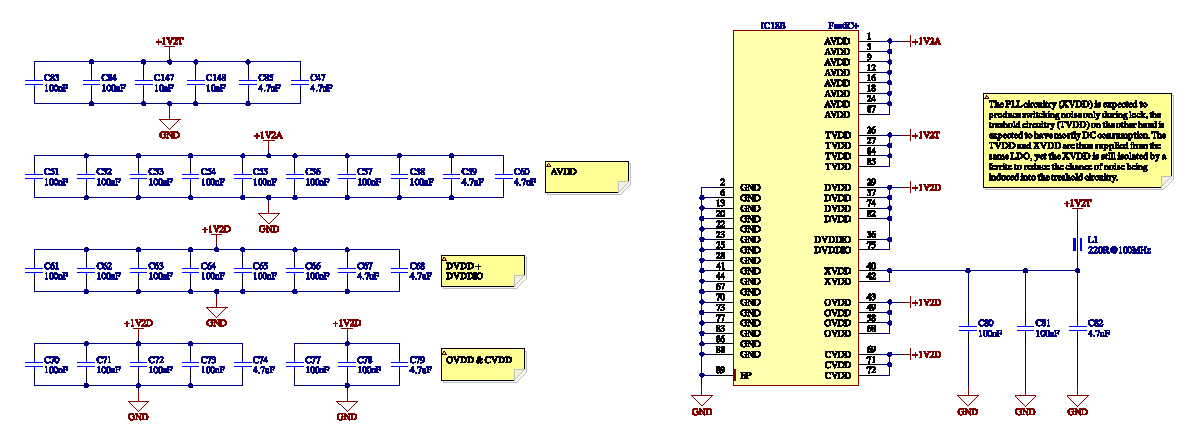
\includegraphics[scale=0.6]{schematic/fastic_power.eps}
    \caption{Schematic of the FastIC+ power}
    \label{fig:fastic_power}
\end{figure}
\FloatBarrier
%
To increase the stability of the internal band gap reference, a \SI{10}{\nano\farad} capacitor has been added to the \verb|VBG| pin.

Both \verb|nRST| (reset of the FastIC+) and \verb|SRST| (reset of the synchronous counter) have been pulled up to the digital supply so that the microcontroller pins in open drain mode can be used to control these pins without the need for voltage translation. 

\FloatBarrier
\begin{figure}[htp!]
    \centering
    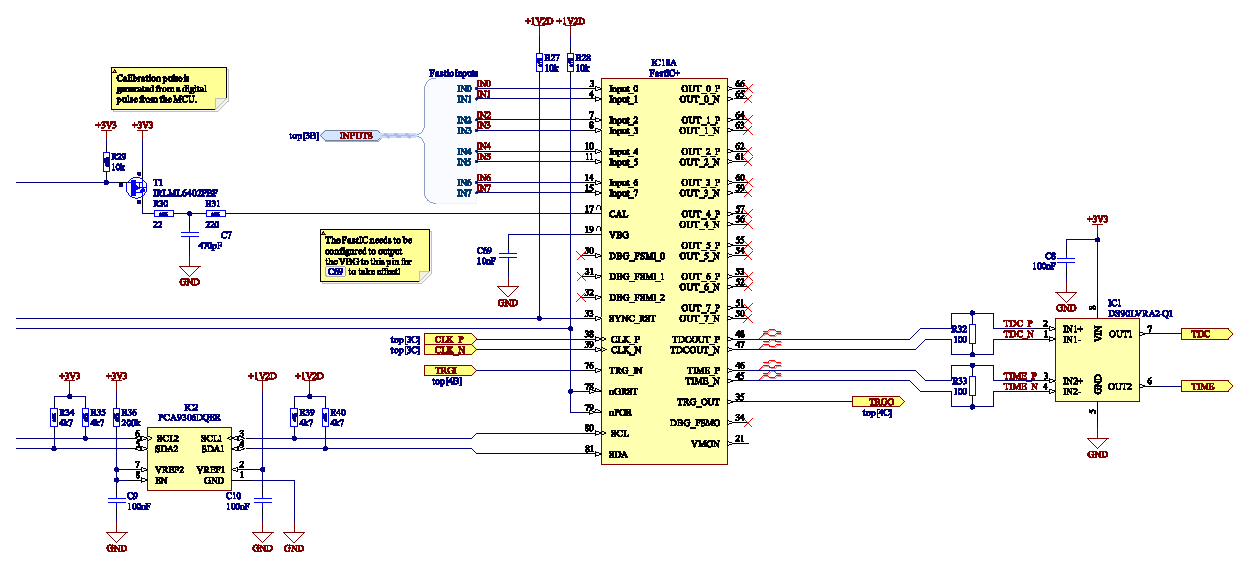
\includegraphics[scale=0.6]{schematic/fastic.eps}
    \caption{Schematic of the FastIC+ logic}
    \label{fig:fastic}
\end{figure}
\FloatBarrier


%
\subsection{I2C communication}
As the FastIC+ voltage domains all run at \SI{1.2}{\volt}, a voltage shifter had to be implemented for communication with the microcontroller over I2C. For this, the PCA9306DQER has been chosen for its miniature X2SON package and sufficent \SI{400}{\kilo\hertz} speed. 
%
\subsection{Calibration pulse generator}
The FastIC+ features a \verb|CAL| input pin used for injecting a test pulse into any of the eight input channels. This pin converts the pulse to current with an internal \SI{70}{\ohm} resistor. The usual shape of such a pulse should resemble a real sensor output, thus a decaying exponential with an amplitude of a few milliamperes and length under a microsecond. To create this pulse, a high side switch has been implemented with series resistance to limit the current and parallel capacitance to recreate the decaying exponential. The transistor gate is driven by a quick digital pulse from the microcontroller, whos length can be adjusted to adjust the current pulse width and by some degree also the amplitude. 
%
\subsection{Voltage monitoring}
%
The \verb|VMON| pin on the ASIC serves for monitoring of the internal analog tresholds and DAC outputs. Since the microcontrollers internal voltage reference has been selected to run at \SI{1.8}{\volt}, a simple non inverting amplifier, with a voltage gain of
%
\begin{equation}
    A_V = \left( 1 + \frac{R41}{R44}\right) = \left( 1 + \frac{\SI{10}{\kilo\ohm}}{\SI{20}{\kilo\ohm}}\right) = 1.5
\end{equation}
%
has been implemented to amplify the \SI{1.2}{\volt} output to the microcontrollers full-scale range and improve the performance. Because the \verb|VMON| output is used only for treshold monitoring, thus only DC voltages, a slow RC filter has been used to reduce the noise coupled to the analog signal.
%
\FloatBarrier
\begin{figure}[htp!]
    \centering
    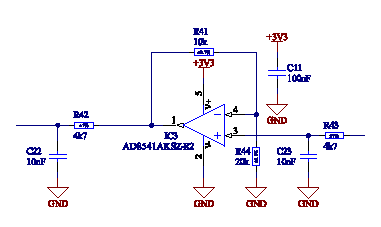
\includegraphics[scale=2]{schematic/fastic_vmon.eps}
    \caption{Schematic of the voltage monitoring amplifier}
    \label{fig:fastic_vmon}
\end{figure}
\FloatBarrier
%
\subsection{High speed outputs}
%
The FastIC+ outputs are realized using the Scalable Low Voltage Signaling standard. SLVS is a alternative to the LVDS, utilizing lower voltages. The transmitter common mode voltage $V_{CMTX}$ being \SI{0.6}{\volt} and the differential voltage $|V_{OD}|$ being \SI{0.2}{\volt} as seen in figure \ref{fig:slvs_voltages}.

\begin{figure}[ht]
	\begin{center}
		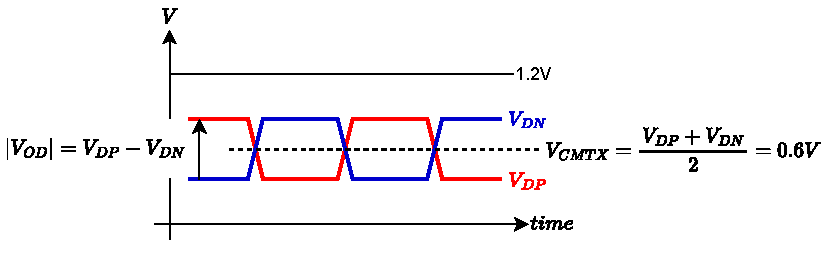
\includegraphics[scale=0.8]{06_SLVS_specs.pdf}
	\end{center}
	\vspace{-5mm}
	\caption{Voltage definition for SLVS transmitter.}
	\label{fig:slvs_voltages}
\end{figure}

A differential output capable of transmitting a pulse whos beginning timestamps the ToA of a photon and length resembles the ToT is present for each channel separately. However, as the readout uses the data digitalized by the internal TDC, these channels are left unconnected and disabled in the chip.

The \verb|TIME| output can either be used to generate a digital pulse whenever any input is received on any of the channels or can be internally connected to the trigger comparator and used for trigger calibration routine, the latter being used in this case. When the pin is not used for calibration, it is disabled to reduce any EMI generated by the fast edges. The \verb|TDCOUT| is the output of the Aurora stream from the transmitter.

Both of the above mentioned pins are connected to the DS90LVRA2 dual channel differential line receiver and terminated by a \SI{100}{\ohm} resistance. This receiver, used to convert the SLVS output to CMOS, has been chosen specifically for its small size, high enough speed but also for its typical propagation delay $t_{pd}$ = \SI{4.4}{\nano\second} to correctly align the data to the sampling clock. Even though it is made to convert LVDS signals, the treshold voltage levels work well with the SLVS standard mentioned above, thus no other special circuitry is needed. 

\subsection{Trigger input and output}
The trigger inputs (used for externally triggering the ASIC) and outputs (outputting the signal from the internal comparator) have been exposed to the user on two SMA connectors. Termination has been placed on these to mitigate any reflections and ESD protection diodes have been added to protect the chip from electrostatic discharge. It's important to note that the ESD diodes add capacitance to the trigger lines, thus degrading (slowing) the trigger edge and introducing a slight delay in the trigger. This either needs to be accounted for when using the readout or the diodes need to be left unassembled at the expense of worse ESD immunity. 
%
\FloatBarrier
\begin{figure}[htp!]
    \centering
    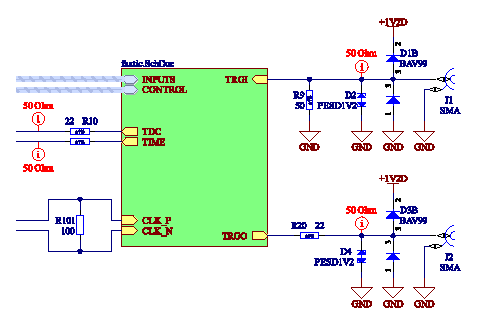
\includegraphics[scale=1.6]{schematic/fastic_top.eps}
    \caption{Schematic of the FastIC+ trigger circuitry}
    \label{fig:schem_fastic_triggers}
\end{figure}
\FloatBarrier

\section{USB}
To supply power to the device and handle communication with the host computer, a USB type C connector has been used.
\FloatBarrier
\begin{figure}[htp!]
    \centering
    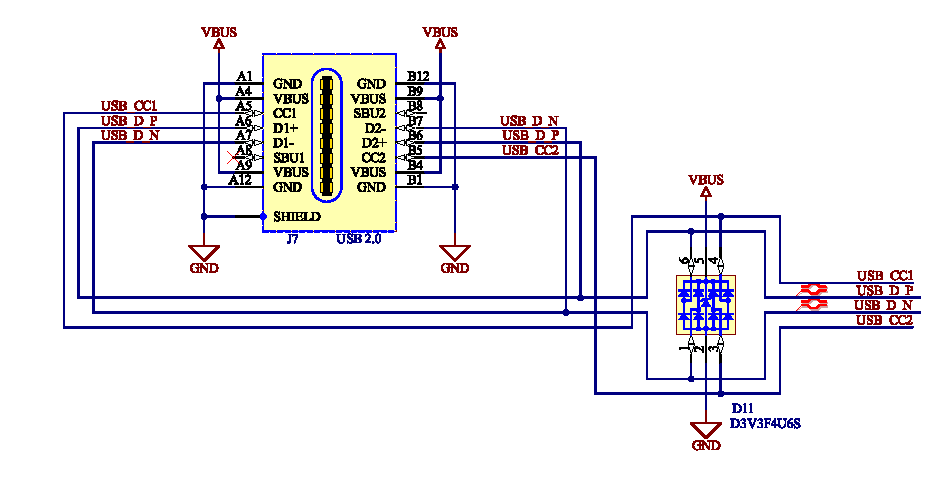
\includegraphics[scale=.75]{schematic/usb_con.eps}
    \caption{Schematic of the USB connector with ESD protection}
    \label{fig:schem_usb_con}
\end{figure}
\FloatBarrier
\subsubsection{External PHY}
Because the combined data rate of the FastIC+ chips of \SI{160}{\mega\bit\per\second} exceeds the USB 1.1 specification, a USB 2.0 (High Speed) was implemented, supporting up to \SI{480}{\mega\bit\per\second} throughput. Unfortunately, the used microcontroller does not integrate the USB 2.0 PHY directly. Instead, it only integrates the necessary logic and interfaces with an external PHY via the ULPI interface. 


A USB3320 interface was chosen as it is well supported by the microcontroller and widely used in countless designs. A \SI{48}{\mega\hertz} crystal oscillator has been used as the external reference clock required for the device to operate. Different crystal frequency selection has been made possible with \SI{0}{\ohm} resistor jumpers. The ULPI connections have been series terminated, to better match the driver output impedance to the cotrolled impedance of the line. 
\FloatBarrier
\begin{figure}[htp!]
    \centering
    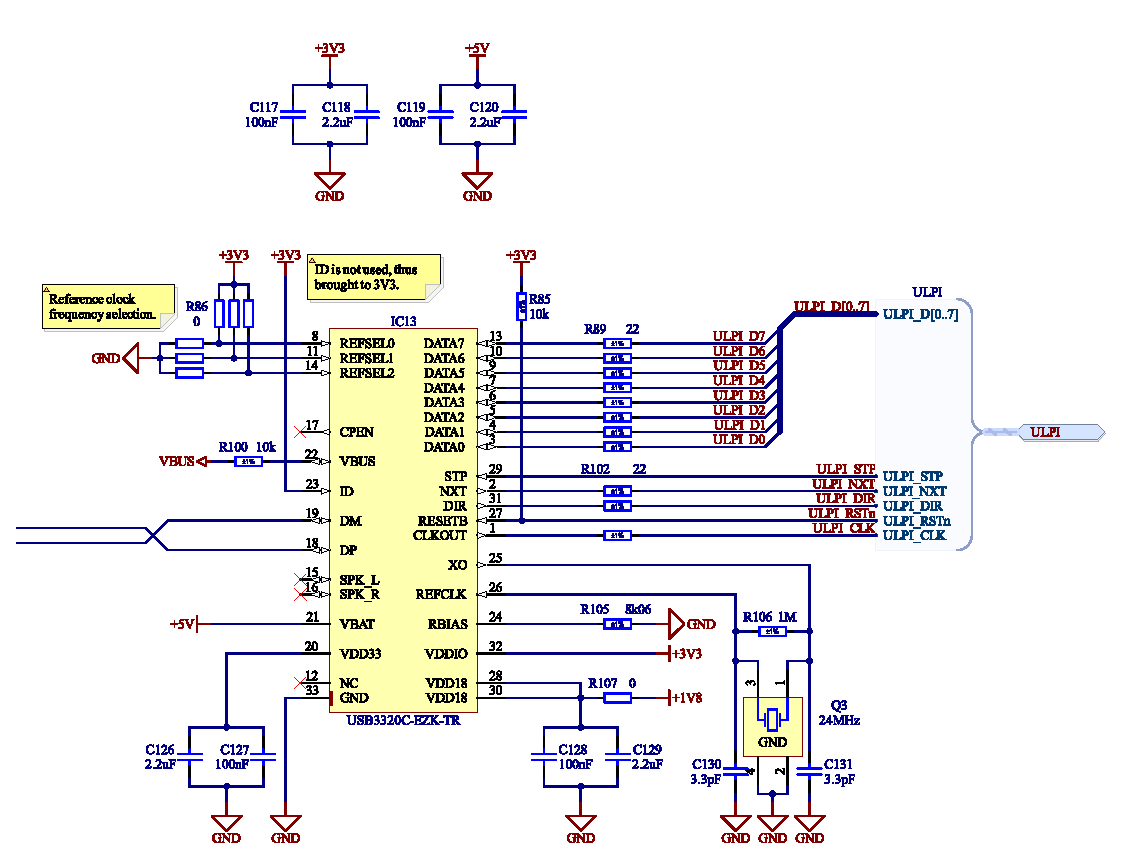
\includegraphics[scale=.68]{schematic/usb.eps}
    \caption{Schematic of the USB}
    \label{fig:schem_usb}
\end{figure}
\FloatBarrier
\subsubsection{Power Delivery}
A FUSB302 chip was added to allow for power limit negotiation with a UCPD capable power source. The chip handles all the necessary signaling and communicates with the MCU via a I2C interface. Optional \SI{5.1}{\kilo\ohm} resistors have been added to passively negotiate the highest power limit, if it would be decided to omit the power delivery functionality and not assemble the FUSB302.
\FloatBarrier
\begin{figure}[htp!]
    \centering
    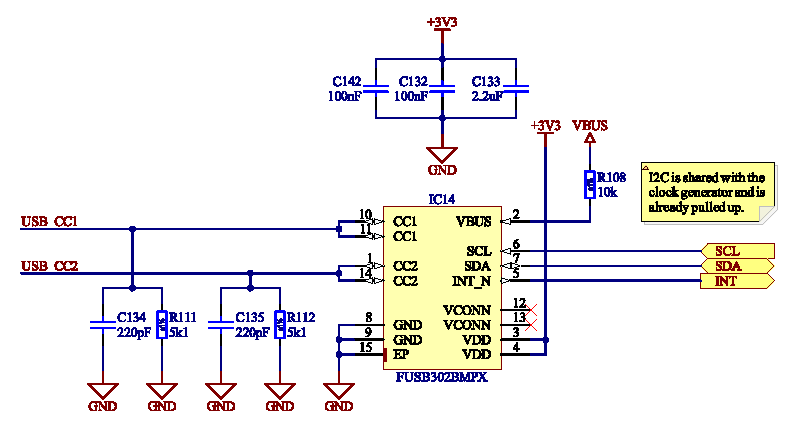
\includegraphics[scale=.9]{schematic/ucpd.eps}
    \caption{Schematic of the USB}
    \label{fig:schem_ucpd}
\end{figure}
\FloatBarrier
\subsection{Clock generation}
For generating the \SI{40}{\mega\hertz} reference clock for both of the FastIC+ chips and the \SI{80}{\mega\hertz} sampling clock for the SPI peripherals, the SI5340 clock synthetizer has been used. It features four outputs with \SI{90}{\femto\second} RMS jitter, supporting both CMOS and differential output. Additionally, each output can be powered by an independent power supply allowing for mixing the \SI{3.3}{\volt} CMOS signals for the microcontroller and differential signals for the FastIC+. A precise \SI{48}{\mega\hertz} crystal oscillator has been used as the reference clock. The chip features both I2C and SPI interface for configuration. I2C was selected to be used in this design.

\FloatBarrier
\begin{figure}[htp!]
    \centering
    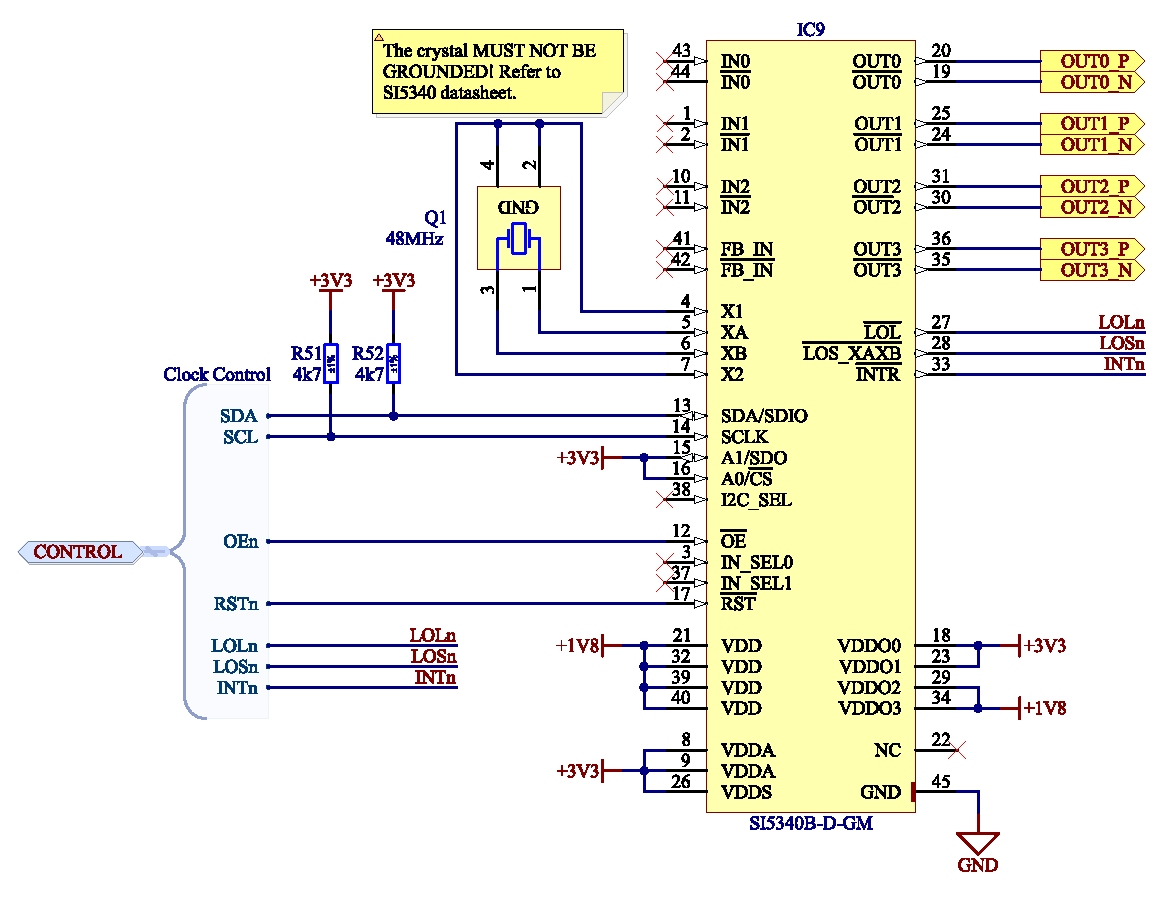
\includegraphics[scale=0.65]{schematic/clock.eps}
    \caption{Schematic of the clock generator}
    \label{fig:schem_clock}
\end{figure}
\FloatBarrier

Since the FastIC+ requiers an SLVS input, which is not supported by the generator a signal divider had to be implemented. This circuit, shown in figure \ref{fig:schem_slvs}, was provided in the datasheet as a good way to lower the voltage levels while keeping the impedance of the lines well matched. 
\FloatBarrier
\begin{figure}[htp!]
    \centering
    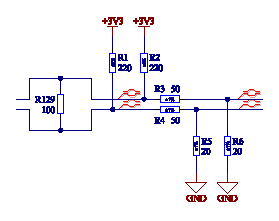
\includegraphics[scale=2]{schematic/slvs.eps}
    \caption{Divider for the LVDS to SLVS conversion}
    \label{fig:schem_slvs}
\end{figure}
\FloatBarrier

\subsection{High Voltage}
All the sensors, which the FastIC+ shall interface with, like SiPMs, PMTs or MCPs need high voltage biasing for their function. To eliminate the need for an external HV supply, an internal one has been implemented using the LT3571. This DC/DC converter, intended for biasing of avalanche photodiodes, is capable of generating up to \SI{75}{\volt} output from a low voltage input. It fully integrates the power switch and regulation along with soft-start and variable switching frequency. This has been set to approximately \SI{1}{\mega\hertz} via \verb|R61|. Higher switching frequency than allows for use of smaller inductance and thus keep the size of the device small. 

\FloatBarrier
\begin{figure}[htp!]
    \centering
    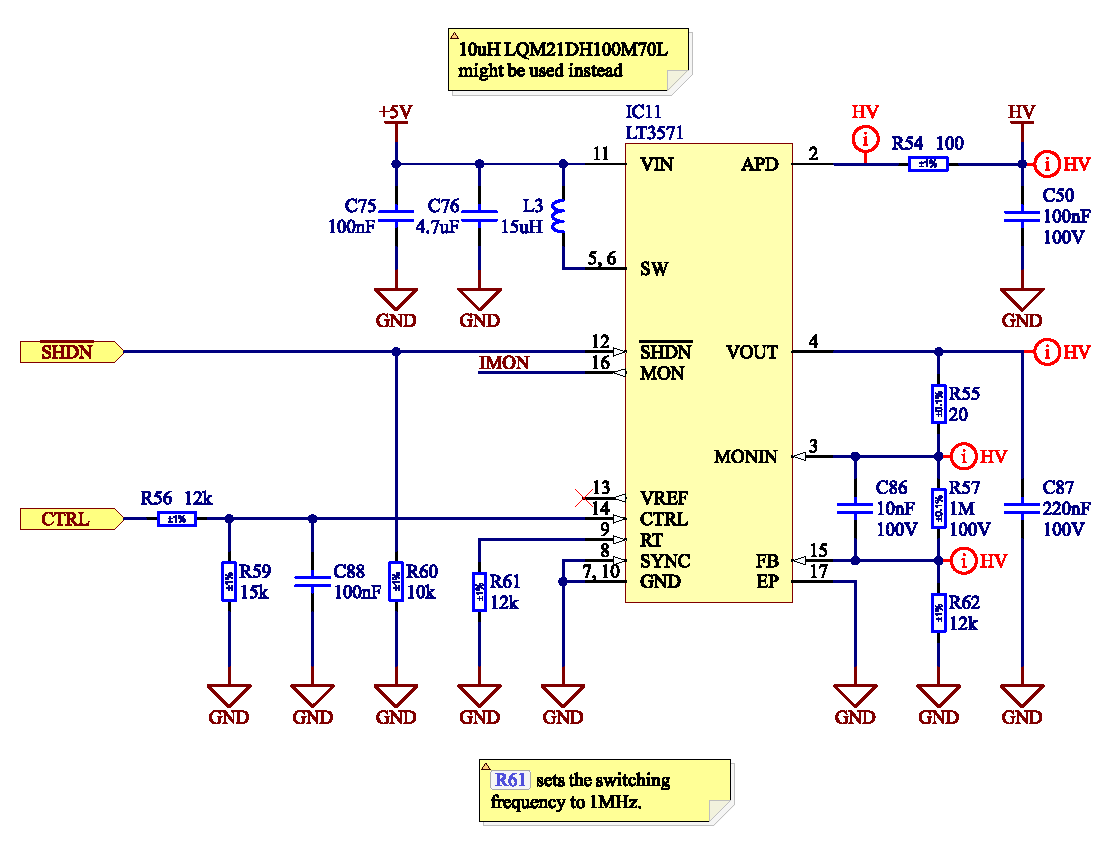
\includegraphics[scale=.65]{schematic/hv.eps}
    \caption{High voltage power supply schematic}
    \label{fig:schem_hv}
\end{figure}
\FloatBarrier

A \verb|CTRL| input is available for adjusting the output with a control voltage. This reference is generated by the MCU DAC and divided by a voltage divider to a suitable \SI{0}{V} -  \SI{1}{V} range. The feedback resistor divider was chosen such that the theoretical maximum output voltage with the \verb|CTRL| pin held at \SI{1}{\volt} is \SI{84.3}{\volt} according to equation \ref{eq:hv_voltage_fb}.

\begin{equation}
V_{MONIN} = (\frac{R57}{R62} + 1) \cdot V_{CTRL} = (\frac{\SI{1000}{\kilo\ohm}}{\SI{12}{\kilo\ohm}} + 1) \cdot \SI{1}{\volt} = \SI{84.3}{\volt}
\label{eq:hv_voltage_fb}
\end{equation}


The current limit resistor has been chosen to limit the APD current to approximately \SI{8}{\milli\ampere} based on the equation \ref{eq:hv_current_limit} mentioned in the datasheet.

\begin{equation}
R_{SENSE} = \frac{\SI{200}{\milli\volt}}{1.2 \cdot I_{APD} + \SI{0.3}{\milli\ampere}} \approx \SI{20}{\ohm}
\label{eq:hv_current_limit}
\end{equation}
%
where $I_{APD}$ is the APD current limit in milliamperes.

To allow for closed loop control with the microcontroller, the output voltage on the APD pin is monitored via a suitable voltage divider with an operational amplifier buffer. For current monitoring, the LT3571 offers the \verb|IMON| pin which sources a current $I_{IMON} = 0.2 \cdot I_{APD}$. This current is than converted to voltage with a \SI{1}{\kilo\ohm} shunt resistor and buffered with an operational amplifier.

\FloatBarrier
\begin{figure}[htp!]
    \centering
    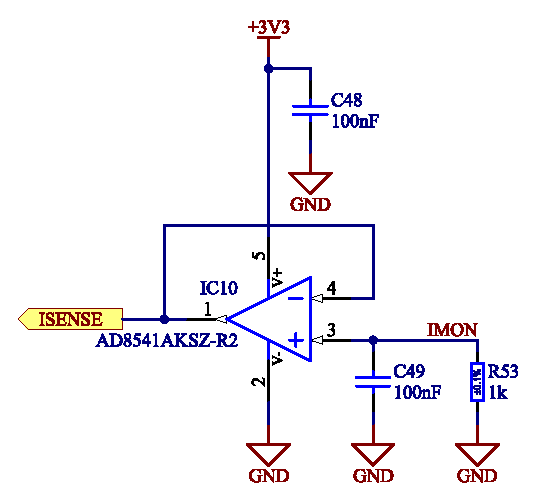
\includegraphics[scale=.8]{schematic/hv_isense.eps}
    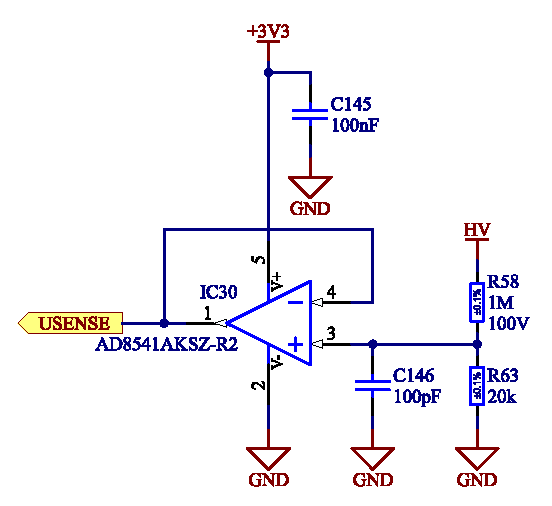
\includegraphics[scale=.8]{schematic/hv_usense.eps}
    \caption{Sensing of the high voltage and current}
    \label{fig:schem_hvsense}
\end{figure}
\FloatBarrier

\subsection{Power}
A DC/DC converter has been implemented to efficiently lower the \SI{5}{\volt} input voltage to the \SI{3.3}{\volt} used by the microcontroller. The \SI{3.3}{\volt} for the analog domain has been generated with a low ripple LDO. The \SI{1.8}{\volt} domain for the USB interface has been derived from the \SI{3.3}{\volt} using an LDO aswell, as efficiency is not required with the low power consumption of \SI{29.4}{\milli\ampere} of the \SI{1.8}{\volt} domain.
\FloatBarrier
\begin{figure}[htp!]
    \centering
    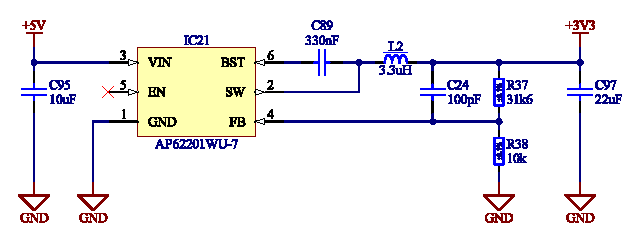
\includegraphics[scale=1]{schematic/power_dcdc.eps}
    \caption{Step down regulator schematic}
    \label{fig:schem_dcdc}
\end{figure}
\FloatBarrier

Power sequencing has been implemented for all the three FastIC+ voltage domains. First, the digital domain supply is activated, followed by the supply for the treshold circuitry and PLL and lastly, the analog domain is supplied. All of these domains are derived from the \SI{3.3}{\volt} using a \SI{1.2}{\volt} LDOs which are sufficient for the low power consumption (\SI{113}{\milli\ampere} per chip) and provide a ripple-free supply for the sensitive treshold circuitry.

\FloatBarrier
\begin{figure}[htp!]
    \centering
    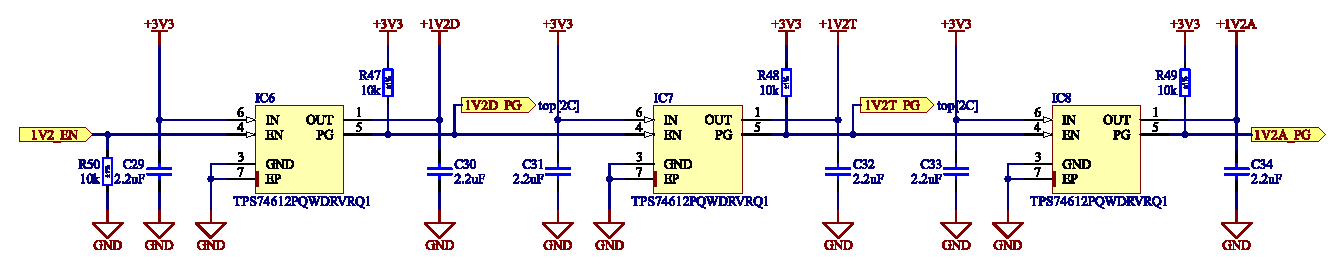
\includegraphics[scale=.55]{schematic/power_fastic.eps}
    \caption{FastIC+ power domain sequencing}
    \label{fig:schem_fastic_power}
\end{figure}
\FloatBarrier

\section{Connector}
For interfacing with the user board, the \SI{9}{\milli\meter} high version of ERM8-020 has been used for its durability, up to 1000 connection cycles, good high speed performance and suitable pin count. This connector carries all the sixteen input channels alongside the high voltage biasing supply. The \SI{3.3}{\volt} supply is also exposed and four pins are dedicated to the user board identification.
%
\subsubsection{Identification pins}
The identification pins serve as an easy way to assign a four bit short ID to a specific user board. This ID can than be used by the software to load a configuration preset defined for the user board. If the userboard designer decides to, the pins ID0 and ID1 can be used as I2C communication lines. A compatible EEPROM can than be assembled on the user board, making it possible to save the full configuration on the user board itself, as well as additional data such as name or a unique ID. If the I2C interface is to be used, all of the ID pins need to be pulled up high by a suitable resistor. At least one of the ID pins has to be high at all times, this means that an ID of \verb|0b0000| is not allowed and in this case, the readout will not recognize a valid user board. 
%
\chapter{Userboard}
The userboard has been developed as a template for the users to get easily started with the readout system. It contains a matrix of 4 $\times$ 4 SiPM sensors as well as an EEPROM for storing the board configuration. The \SI{9}{\milli\meter} high ERF8-020 connector has been chosen for the user board to match the counterpart present on the readout and allow enough clearance between the assembled readout board and user board.

\section{Sensors}
The footprint for a generic THT SiMPs has been implemented on the board. Each SiPM is powered from the HV plane and the input is filtered with a dual RC low pass to eliminate a possibility of cross triggering of the sensors. 

\FloatBarrier
\begin{figure}[htp!]
    \centering
    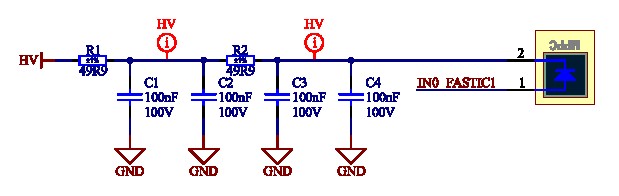
\includegraphics[scale=1.2]{schematic/sipm.eps}
    \label{fig:sipm}
\end{figure}
\FloatBarrier

\section{EEPROM}
The 24AA04T-I/OT \SI{4}{\kilo\bit} EEPROM has been used on the user board for the configuration storage. It has been selected for the low price and sufficient capacity. 



\newpage
\chapter{PCB design}
Special care had to be taken when designing the PCB to keep in mind the correct design practices for propper power integrity, signal integrity and high speed design.

First a suitable stackup was chosen. In this case, it was decided to proceed with an eight layer stackup as shown in table \ref{tab:stackup}. 
\FloatBarrier
\begin{table}[]
    \caption{PCB stackup}
    \begin{tabular}{|l|l|l|}
    \hline
    \multicolumn{1}{|c|}{\textbf{Layer}} & \multicolumn{1}{c|}{\textbf{Name}} & \multicolumn{1}{c|}{\textbf{Thickness}} \\ \hline
    1                                    & L1 - Top copper                    & \SI{0.018}{\milli\meter}                                   \\ \hline
                                         & Dielectric - PR2116                & \SI{0.120}{\milli\meter}                                   \\ \hline
    2                                    & L2 - Ground plane                  & \SI{0.035}{\milli\meter}                                   \\ \hline
                                         & Dielectric - FR4 core              & \SI{0.200}{\milli\meter}                                   \\ \hline
    3                                    & L3 - Power plane                   & \SI{0.035}{\milli\meter}                                   \\ \hline
                                         & Dielectric - PR2116                & \SI{0.120}{\milli\meter}                                   \\ \hline
                                         & Dielectric - PR2116                & \SI{0.120}{\milli\meter}                                   \\ \hline
    4                                    & L4 - Signal layer                  & \SI{0.035}{\milli\meter}                                   \\ \hline
                                         & Dielectric - FR4 core              & \SI{0.200}{\milli\meter}                                   \\ \hline
    5                                    & L5 - Signal layer                  & \SI{0.035}{\milli\meter}                                   \\ \hline
                                         & Dielectric - PR2116                & \SI{0.120}{\milli\meter}                                   \\ \hline
                                         & Dielectric - PR2116                & \SI{0.120}{\milli\meter}                                   \\ \hline
    6                                    & L6 - Power plane                   & \SI{0.035}{\milli\meter}                                   \\ \hline
                                         & Dielectric - FR4 core              & \SI{0.200}{\milli\meter}                                   \\ \hline
    7                                    & L7 - Ground plane                  & \SI{0.035}{\milli\meter}                                   \\ \hline
                                         & Dielectric - PR2116                & \SI{0.120}{\milli\meter}                                   \\ \hline
    8                                    & L8 - Bottom copper                 & \SI{0.018}{\milli\meter}                                   \\ \hline
    \end{tabular}
    \label{tab:stackup}
\end{table}
\FloatBarrier
The layers 2 and 3 and layers 6 and 7 were completly dedicated as ground and power planes. This, in combination with relatively thin dielectric in between, creates an inherent capacitive coupling between the planes proportional to the plane area and spacing which helps the power integrity of the device. For a board of size $\SI{50}{\milli\meter} \times \SI{50}{\milli\meter}$, which is the case for the readout, and the stackup mentioned, this capacitance can be estimated with an equation for a parallel plate capacitor to be
%
\begin{equation}
C = \varepsilon_0 \cdot \varepsilon_r \cdot \frac{S}{d} = \SI{8.85e-12}{\farad\per\meter} \cdot 4.2 \cdot \frac{\SI{2500}{\milli\meter\squared}}{\SI{0.2}{\milli\meter}} = \SI{465}{\pico\farad}
\end{equation}
%
Leaving the planes for solid planes only also keeps the impedance of the planes minimal which reduces the voltage drops in the planes. The layers 4 and 5 were also mostly kept as planes, although some connections needed to be routed through these because of the very high board density. While routing in these layers, care was taken not to cross possible return current paths of the planes with another trace, which could result in a much bigger current loop and an increase in EMI. Layers 1 and 8, the top and bottom copper, were used mainly for routing of all the signals. Since both of the layers have a ground reference underneath, both of them can and were used for routing of the high speed lines with defined impedance. 
%
\section{High speed signals}
To mitigate any possible reflections on the high speed lines which carry high frequency signals, the charasteristic impedance of all of these was calculated to match the driver impedance. In case of the differential signals, the differential impedance of the lines was optimized to be \SI{100}{\ohm}, aside from the USB which requires a \SI{90}{\ohm} differential impedance. For the single ended lines, the target impedance was \SI{50}{\ohm}. The widths of the lines along with the spacing for the differential lines were calculated using the Altium Designer impedance calculation tool and double checked using the manufacturers impedance calculation tool. These calculations yilded the width $W_{USB} = \SI{0.183}{\milli\meter}$ and spacing $S_{USB} = \SI{0.2}{\milli\meter}$ for the USB differential pair, the width $W_{DIFF} = \SI{0.15}{\milli\meter}$ and spacing $S_{DIFF} = \SI{0.2}{\milli\meter}$ for the rest of the differential pairs and the width $W_{SE} = \SI{0.182}{\milli\meter}$ for all of the single-ended high speed lines. The widths and spacings were obeyed during the routing to keep the tracks impedance as close to the target impedance as possible.

\section{BGA fanout}


\section{Power integrity}

The two concepts described above were designed and manufactured keeping in mind the required performance. The final PCBs can be seen on the images bellow. 
\newpage
\FloatBarrier
\begin{figure}[htp!]
    \centering
    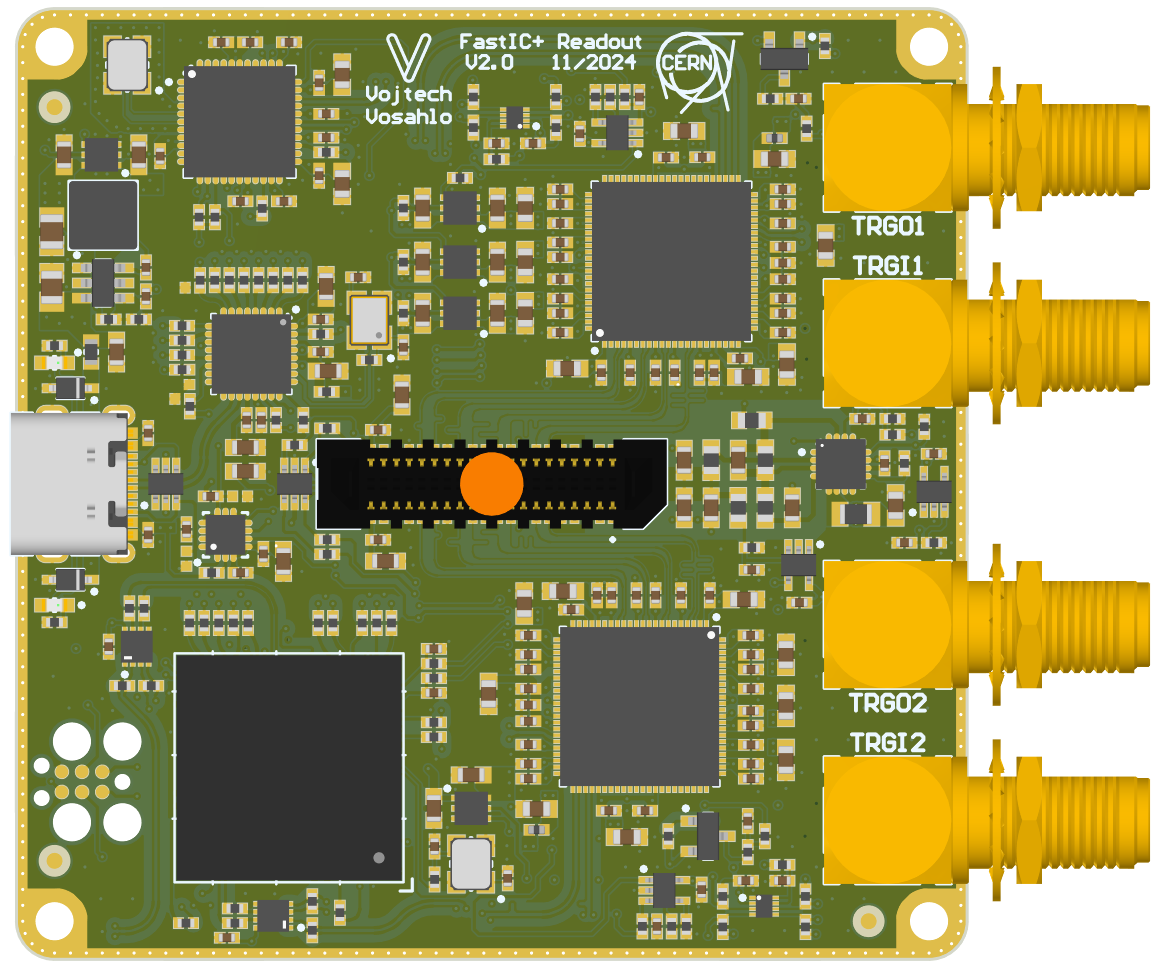
\includegraphics[height=5.2cm]{readout_3d-top.png}
    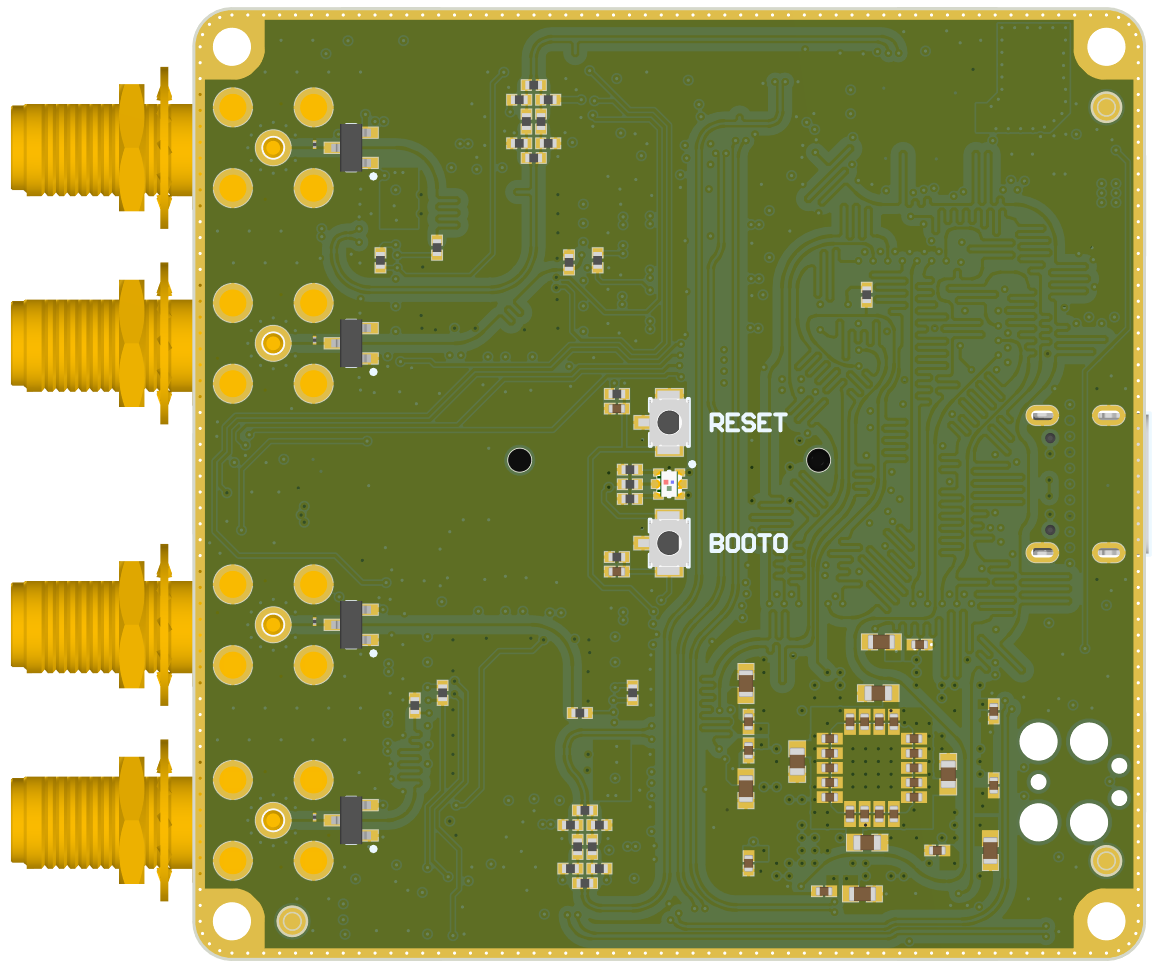
\includegraphics[height=5.2cm]{readout_3d-bottom.png}
    \caption{Readout PCB}
    \label{fig:readout_3d}
\end{figure}
\FloatBarrier

\FloatBarrier
\begin{figure}[htp!]
    \centering
    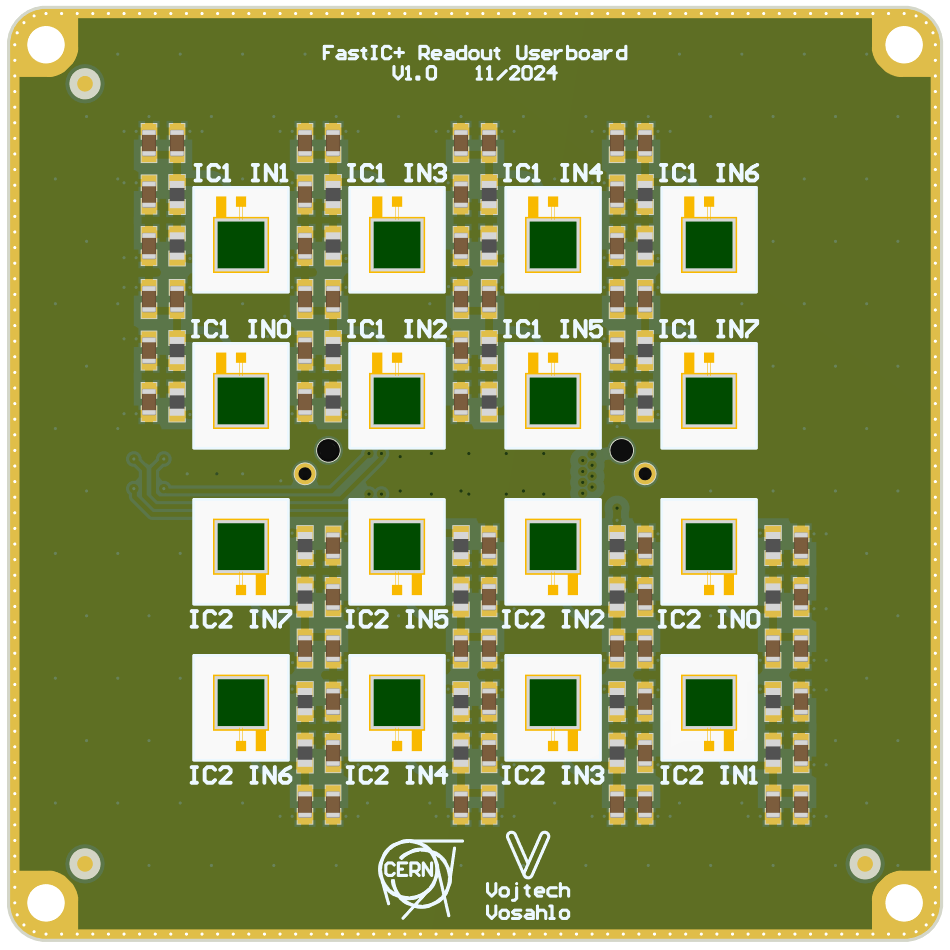
\includegraphics[height=5.2cm]{userboard_3d-top.png}
    \hspace{1.8cm}
    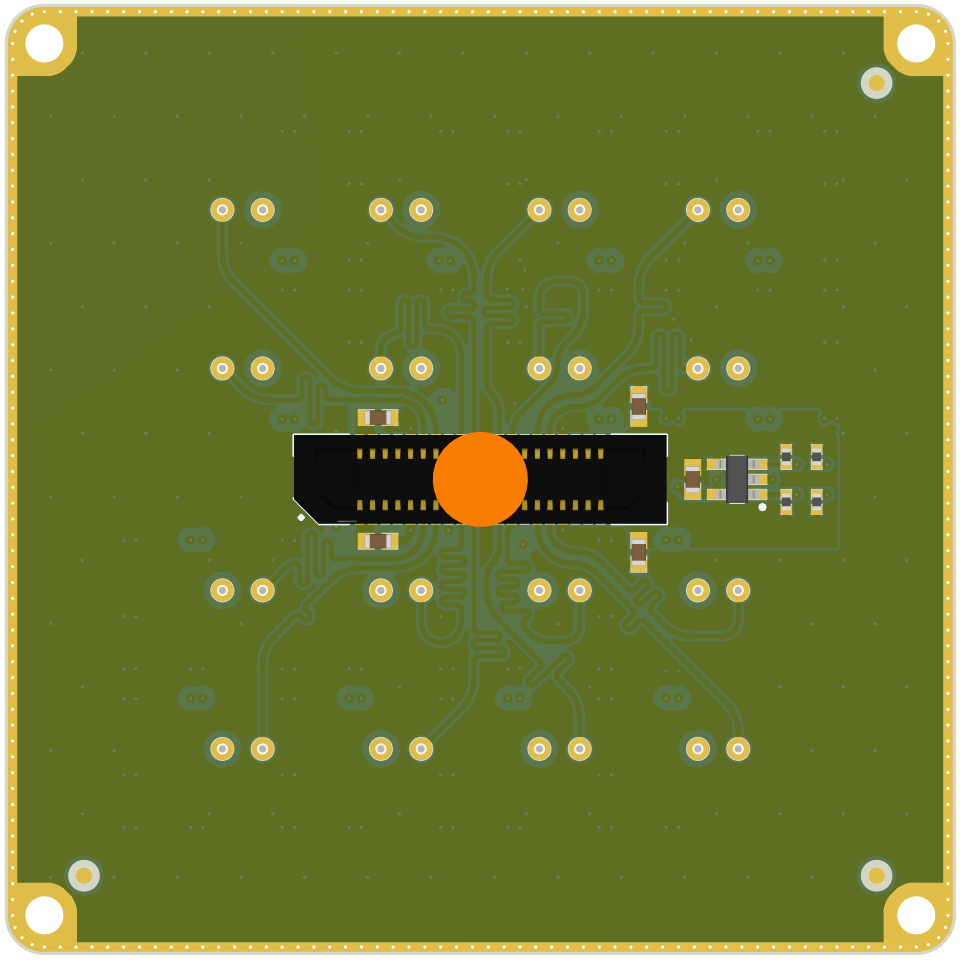
\includegraphics[height=5.2cm]{userboard_3d-bottom.png}
    \caption{Userboard PCB}
    \label{fig:userboard_3d}
\end{figure}
\FloatBarrier
